
%%\include{Begin}

\section{バス内(行き)}

\begin{tabular}{p{2zw}rp{38zw}}
  日時 & : & 2019年4月5日(金) 12:10 $\sim$ 14:40\\ %未定
  場所 & : & バス
\end{tabular}

\subsection{目的}
新入生の緊張をほぐし,仲を深める.


\subsection{タイムスケジュール}
% 時刻は必ず4桁(00:00)で書くこと!!!
\begin{longtable}{p{3zw}p{39zw}}
  12:20 & \textbf{◎ バス出発 } \\
        & \ \ \textbullet \ \ 連絡係(伊崎,吉田,江川)は受付との乗車チェックが終わり次第,乗車チェックが完了したことを報告LINEに連絡する \\
        & \ \ \textbullet \ \ 全車の乗車チェックが終わり次第,出発する \\
        & \ \ \textbullet \ \ 連絡係はバスが出発したことを報告LINEに連絡する \\
	    & \ \ \textbullet \ \ 連絡係はバスの状況を見て話し始める \\\\

        & \textbf{◎ 司会者挨拶,自己紹介} \\     
        & \textbf{◎これからの流れ説明 } \\
        & \textbf{◎ バス内諸注意,スタッフ紹介} \\   
        & \textbf{◎ 流れ説明} \\
        
  12:45 & \textbf{◎ 道の駅(風良里)到着} \\
	    & \ \  \textbullet \ \ 補助席に座ってる人が先に降りる \\
	    & \ \  \textbullet \ \ スタッフは新入生の奇行に目を配る \\
	    & \ \  \textbullet \ \ バス連絡係は報告slackで到着の旨を連絡する \\\\

  12:55 & \textbf{◎ 乗車開始} \\
  	    & \ \  \textbullet \ \ 気分が悪い人がいないか確認する(もしいた場合は救護車に移動してもらう) \\
	    & \ \  \textbullet \ \ 司会者は新入生に隣の席の人がいるか確認してもらい,人数を確認する \\
	    & \ \  \textbullet \ \ バス連絡係はバス司会は報告slackで乗車開始の旨を連絡する \\\\
	
  13:00 & \textbf{◎ 道の駅(風良里)出発} \\
	    & \ \  \textbullet \ \ 運転手に乗車確認を伝え順次出発する\\
	    & \ \  \textbullet \ \ バス連絡係は報告slackで出発の旨を連絡する\\\\

        & \textbf{◎ 教員紹介} \\ 
        & \textbf{◎ バス内企画 その1} \\
      	& \ \  \textbullet \ \ 自己紹介ゲーム \\
        & \textbf{◎ バス内企画 その2} \\
		& \ \  \textbullet \ \ 方言当てゲーム\\
        
  14:00 & \textbf{◎ あぐり窪川到着} \\
	    & \ \  \textbullet \ \ 補助席に座ってる人が先に降りる \\
	    & \ \  \textbullet \ \ スタッフは新入生の奇行に目を配る \\
	    & \ \  \textbullet \ \ バス連絡係は報告slackで到着の旨を連絡する \\\\

  14:25 & \textbf{◎ 乗車開始} \\
	    & \ \  \textbullet \ \ 気分が悪い人がいないか確認する(もしいた場合は救護車に移動してもらう) \\
	    & \ \  \textbullet \ \ 司会者は新入生に隣の席の人がいるか確認してもらい,人数を確認する \\
	    & \ \  \textbullet \ \ バス連絡係はバス司会LINEで乗車開始の旨を連絡する \\\\

  14:30 & \textbf{◎ あぐり窪川出発} \\
	    & \ \  \textbullet \ \ 運転手に乗車確認を伝え順次出発する \\
	    & \ \  \textbullet \ \ バス連絡係は報告LINEで出発の旨を連絡する \\\\

        & \textbf{◎ バス内企画 その3} \\
	    & \ \  \textbullet \ \ 100分の1ゲーム \\
  
  15:10 & \textbf{◎ 幡多到着5分前} \\
	    & \ \  \textbullet \ \ タイムライン上は到着5分前だが本番は山道に入ったところでもうすぐ着くというアナウンスをする \\
        & \ \  \textbullet \ \ 名札をつけていることを確認してもらい,野外炊事のグループを名札で確認をしてもらう \\
        & \ \  \textbullet \ \ トイレ,荷物について説明する \\
        & \ \  \textbullet \ \ 入所式の並び方を説明する \\
	    & \ \  \textbullet \ \ バス連絡係は報告slackで山道に入った旨を連絡する \\\\

  15:15 & \textbf{◎ 幡多到着} \\
        & \ \ \textbullet \ \ 到着後スタッフは速やかに降りて荷下ろしをする \\
	    & \ \ \textbullet \ \ 3号車は2号車の荷下ろしの手伝いをする \\
	    & \ \ \textbullet \ \ 道の駅(風良里)とあぐり窪川の休憩とは違い全員がバスから降りるので前から順に速やかに降りてもらう \\
        & \ \ \textbullet \ \ 到着した旨を報告slackに連絡する \\\\
\end{longtable}

%%\subsection{内容}
\subsection{人員配置(図\ref{fig:bus_memberHaichi1},\ref{fig:bus_memberHaichi2},参照)}
○1号車
\begin{itemize}
\item 司会:藤田,北村
\item 補助: 伊崎,斎藤,生野,高島,高橋(慎),石野
\end{itemize}
○2号車
\begin{itemize}
\item 司会:中島,高橋(龍)
\item 補助: 吉田,渡辺,立岩,日下,真壁,新田

\end{itemize}
○3号車
\begin{itemize}
\item 司会:丸田,塩谷
\item 補助: 青山,新川,角原,小谷,別役,東,江川

\end{itemize}


\subsection{トランク内荷物配置図}
\begin{figure}[H]
\begin{tabular}{lr}
\begin{minipage}{1.0\textwidth}
  \begin{center}
  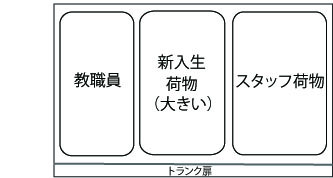
\includegraphics[width=8cm]{./06/baggage_place_1.eps}
  \caption{トランク内荷物配置図(1,2,3号車)}
  \end{center}
\end{minipage}
\end{tabular}
\end{figure}

\subsection{必要物品}
\begin{itemize}
\item 酔い止め薬:各バス1箱
\item エチケット袋:各バス2枚
\item 紙コップ:各バス5個
\item 水(常温):各バス500ml(1本)
\item キッチンタイマー
\item 100分の1ゲームの商品:野外炊事に使用する調味料3種類*3セット
\end{itemize}

\subsection{備考}

\begin{itemize}
\item 司会のどちらが報告slackに連絡を入れるか,各号車ごとに事前に決めておく
\item 先遣隊,他のバス,後遣隊等と随時連絡を取り合う
\item 新入生の体調確認を忘れない
\end{itemize}


%%\include{End}
